\documentclass[11pt,a4paper]{article}
\usepackage{../../common/preamble}

\begin{document}

\begin{center}
    {\LARGE \textbf{Сжатие данных}}\\[0.2cm]
    \rule{\textwidth}{1pt}
\end{center}

\section{Математический ликбез}

\subsection{Принцип Дирихле}

В комбинаторике базовый \textbf{принцип Дирихле} формулируется следующим образом:
\begin{quote}
\textit{Если $n$ предметов разложены по $m$ ящикам, и при этом $n > m$, то хотя бы в одном ящике окажется не менее двух предметов.}
\end{quote}

В математике этот принцип формулируется на языке отображений:
\begin{definitionbox}{Принцип Дирихле для конечных множеств}
Пусть $A$ и $B$ --- конечные множества, причем их мощности удовлетворяют неравенству $|A| > |B|$. Тогда не существует инъективного отображения $f\colon A \to B$.

Иными словами, для любой функции $f\colon A \to B$ неизбежно найдутся хотя бы два различных элемента $x, y \in A$ ($x \neq y$), таких что:
$$f(x) = f(y)$$
\end{definitionbox}

\subsection{Сумма геометрической прогрессии}

\textbf{Геометрической прогрессией} называется числовая последовательность $(b_n)$, каждый член которой, начиная со второго, получается из предыдущего умножением на фиксированное ненулевое число $q$ (знаменатель прогрессии):
$$b_n = b_1 \cdot q^{n-1}$$

Сумма первых $n$ членов геометрической прогрессии $S_n = \sum\limits_{k=1}^n b_k$ при $q \neq 1$ вычисляется по формуле:
$$S_n = b_1 \frac{q^n - 1}{q - 1}$$

\section{Основные понятия сжатия данных}

Сжатие данных необходимо для двух практических целей:
\begin{enumerate}
    \item Экономия емкости на внешних накопителях
    \item Увеличение скорости передачи данных по компьютерным сетям
\end{enumerate}

Сжать данные --- значит уменьшить их информационный объем за счет сокращения длины двоичного кода с использованием \textbf{избыточности информации}.

\subsection{Базовый пример сжатия по известной избыточности}
Пусть текстовый файл объемом $10\text{ Кбайт}$ ($10\,240$ символов в 8-битной кодировке) содержит всего четыре различных символа: латинские буквы \texttt{A, B, C} и \texttt{пробел}. Для различения 4 вариантов достаточно $i = \log_2 4 = 2$ бита:
$$\texttt{A} \to 00_2, \quad \texttt{B} \to 01_2, \quad \texttt{C} \to 10_2, \quad \text{\textvisiblespace} \to 11_2$$
Строка \texttt{ABA CABABA} (10 байт) превратится в цепочку из 20 бит:
$$\texttt{00010011100001000100}_2$$
Чтобы адресат мог раскодировать сообщение, файл снабжается \textbf{заголовком}:
\begin{itemize}
    \item 1-й байт --- количество используемых символов ($N = 4 \implies 00000100_2$).
    \item Следующие $N = 4$ байта --- их ASCII-коды: \texttt{A} (65), \texttt{B} (66), \texttt{C} (67), \textvisiblespace\ (32).
\end{itemize}
Заголовок занимает $1 + 4 = 5$ байт. Объем сжатого файла:
$$V_{\text{сжат}} = 5 + \frac{10\,240 \cdot 2}{8} = 2565 \text{ байт}$$

\begin{definitionbox}{Коэффициент сжатия и сжатие без потерь}
\textbf{Коэффициент сжатия} $k$ --- это отношение размеров исходного и сжатого файлов:
$$k \defeq \frac{V_{\text{исх}}}{V_{\text{сжат}}}$$
\textbf{Сжатие без потерь} --- такое уменьшение объема закодированных данных, при котором исходные данные восстанавливаются из кода с абсолютной побитовой точностью ($X' = X$).
\end{definitionbox}

\begin{theorembox}{О невозможности универсального сжатия}
Не существует алгоритма сжатия без потерь, способного уменьшить размер абсолютно любого файла длины $N$ бит хотя бы на 1 бит.
\tcblower
\textbf{Доказательство:}  
Из комбинаторных соображений очевидно, что множество всех двоичных файлов длины ровно $N$ бит содержит $|A| = 2^N$ различных цепочек.

Если алгоритм сжимает каждый такой файл хотя бы на 1 бит, то результат будет иметь длину от $0$ до $N-1$ бит. Общее количество таких сжатых файлов равно:
$$|B| = \sum_{j=0}^{N-1} 2^j = 2^N - 1$$

Так как алгоритм обратим, каждому исходному файлу из $A$ должен соответствовать уникальный файл из $B$. Однако $|A| = 2^N > |B| = 2^N - 1$. По принципу Дирихле неизбежно найдутся два разных исходных файла, которые превратятся в один и тот же сжатый файл, что делает однозначное декодирование невозможным. Что и требовалось доказать.
\end{theorembox}

\section{Алгоритм RLE (Run Length Encoding)}

Применяется, когда в данных присутствуют длинные цепочки одинаковых байтов.

\subsection{Базовый алгоритм RLE}

Записывается пара: \texttt{[количество\_повторений, код\_символа]}.  

\textit{Пример:} 100 букв \texttt{А} (код 192) и 100 букв \texttt{Б} (код 193) в 8-битной кодировке занимают 200 байт. В RLE они кодируются всего 4 байтами:
$$\underbrace{01100100_2}_{100} \; \underbrace{11000000_2}_{\text{А}} \quad \underbrace{01100100_2}_{100} \; \underbrace{11000001_2}_{\text{Б}} \implies k = \frac{200}{4} = 50$$

\subsection{Модифицированный алгоритм RLE}

\textbf{Проблема:} Если в файле нет последовательностей одинаковых символов, базовый RLE удвоит объем файла, дублируя счетчик \texttt{1} перед каждым символом.  

\textbf{Решение:} Использование \textbf{управляющего байта}:
\begin{itemize}
    \item \textbf{Старший бит = 1:} признак повтора. Оставшиеся 7 бит --- число повторений. За управляющим байтом следует ровно \textbf{один} байт данных.
    \item \textbf{Старший бит = 0:} признак неповторяющейся цепочки. Оставшиеся 7 бит --- длина серии. За управляющим байтом следует указанное число байтов данных \textbf{без изменений}.
\end{itemize}

\textit{Пример:} Последовательность из 5 байт
$$\underbrace{10001111_2}_{\text{повтор } 15} \quad \underbrace{11000000_2}_{\text{код А}} \quad \underbrace{00000010_2}_{\text{взять } 2} \quad \underbrace{11000001_2}_{\text{код Б}} \quad \underbrace{11000010_2}_{\text{код В}}$$
распаковывается в 17 символов: \texttt{АААААААААААААААБВ}.

\section{Префиксные коды и условие Фано}

При передаче информации без использования специальных символов-разделителей (пробелов или пауз - как в азбуке Морзе) поток элементарных сигналов поступает на приемник непрерывной битовой цепочкой. Естественным образом возникает вопрос: \textbf{как однозначно разделить поток на отдельные символы?}

\subsection{Классификация кодов и условие однозначного декодирования}

Пусть задан исходный алфавит $\Sigma = \{s_1, s_2, \dots, s_M\}$. Каждому символу $s_i$ ставится в соответствие непустое кодовое слово $\vec{c}_i \in \{0, 1\}^+$ длины $l_i = |\vec{c}_i|$.

\begin{definitionbox}{Однозначно декодируемый код}
Код $C = \{\vec{c}_1, \dots, \vec{c}_M\}$ называется \textbf{однозначно декодируемым}, если любая конечная двоичная последовательность может быть сопоставлена не более чем одной исходной последовательности символов:
$$\vec{c}_{i_1}\vec{c}_{i_2}\dots\vec{c}_{i_k} = \vec{c}_{j_1}\vec{c}_{j_2}\dots\vec{c}_{j_m} \implies (k = m) \land (\forall t \hookrightarrow i_t = j_t)$$
\end{definitionbox}

\textit{Антипример:} Код $A \to \texttt{0}$, $B \to \texttt{01}$, $C \to \texttt{10}$. Последовательность \texttt{010} неоднозначна: она может быть прочитана как $AB$ (\texttt{0} + \texttt{10}) или как $BC$ (\texttt{01} + \texttt{0}). Этот код не является однозначно декодируемым.

\subsection{Прямое и обратное условие Фано}

\begin{definitionbox}{Прямое условие Фано (Префиксный код)}
Код называется \textbf{префиксным} (и говорят, что он удовлетворяет \textit{прямому условию Фано}), если ни одно кодовое слово не является началом (префиксом) любого другого кодового слова:
$$\forall i \neq j \hookrightarrow \vec{c}_i \not\sqsubseteq \vec{c}_j$$
\end{definitionbox}

\begin{definitionbox}{Обратное условие Фано (Постфиксный код)}
Код называется \textbf{постфиксным} (и говорят, что он удовлетворяет \textit{обратному условию Фано}), если ни одно кодовое слово не является концом (суффиксом) любого другого кодового слова.
\end{definitionbox}

\begin{questionbox}{Почему в технике чаще используют прямое\, а не обратное условие Фано?}
И префиксный, и постфиксный коды гарантируют однозначность декодирования. Но чаще на практике используют только префиксный. Почему?
\tcblower
\textbf{Ответ:} Постфиксный код требует чтения сообщения \textbf{справа налево} (с конца).  
Чтобы декодировать первое слово, приемник обязан дождаться приема \textbf{всего файла целиком}. Прямое же условие Фано позволяет декодировать символы в реальном времени: как только очередная цепочка бит совпала со словом, символ сразу можно выписывать.
\end{questionbox}

\subsection{Геометрическая интерпретация}

Любой двоичный префиксный код взаимно однозначно отображается на помеченное корневое бинарное дерево:
\begin{itemize}
    \item Переход по левому ребру соответствует биту \texttt{0}, по правому --- биту \texttt{1}.
    \item Кодовое слово определяется путем от корня к соответствующему узлу.
\end{itemize}

\begin{theorembox}{О листьях}
Код удовлетворяет прямому условию Фано тогда и только тогда, когда \textbf{все кодовые слова расположены в листьях дерева} (т.е. у них нет потомков).
\end{theorembox}

Например, код $A \to \texttt{00}$, $B \to \texttt{01}$, $C \to \texttt{10}$, $D \to \texttt{110}$, $E \to \texttt{111}$ можно представить следующим деревом:

\begin{center}
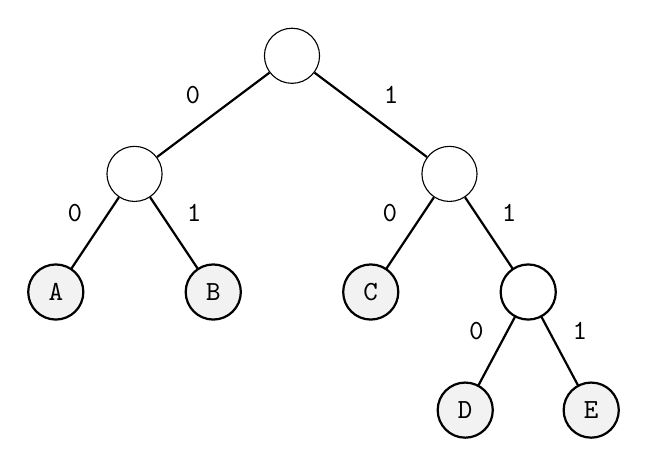
\begin{tikzpicture}[
    level 1/.style={sibling distance=40mm},
    level 2/.style={sibling distance=20mm},
    level 3/.style={sibling distance=16mm},
    every node/.style={circle, draw, minimum size=0.7cm, inner sep=1pt},
    edge from parent/.style={draw, thick}
]
    \node (root) {}
        child {
            node {}
            child { node [fill=black!5] {\texttt{A}} edge from parent node [above left, draw=none] {\texttt{0}} }
            child { node [fill=black!5] {\texttt{B}} edge from parent node [above right, draw=none] {\texttt{1}} }
            edge from parent node [above left, draw=none] {\texttt{0}}
        }
        child {
            node {}
            child { node [fill=black!5] {\texttt{C}} edge from parent node [above left, draw=none] {\texttt{0}} }
            child {
                node {}
                child { node [fill=black!5] {\texttt{D}} edge from parent node [above left, draw=none] {\texttt{0}} }
                child { node [fill=black!5] {\texttt{E}} edge from parent node [above right, draw=none] {\texttt{1}} }
                edge from parent node [above right, draw=none] {\texttt{1}}
            }
            edge from parent node [above right, draw=none] {\texttt{1}}
        };
\end{tikzpicture}
\end{center}

\subsection{Неравенство Крафта-Макмиллана}

Возникает вопрос: какими могут быть длины кодовых слов $\{l_1, l_2, \dots, l_M\}$, чтобы префиксный код гарантированно существовал? Исчерпывающий ответ дает следующая теорема:

\begin{theorembox}{Неравенство Крафта}
Для существования $D$-ичного префиксного кода с набором длин кодовых слов $\{l_1, l_2, \dots, l_M\}$ необходимо и достаточно, чтобы выполнялось неравенство:
$$\sum_{i=1}^M D^{-l_i} \le 1$$

Для двоичного алфавита ($D = 2$):
$$\sum_{i=1}^M \frac{1}{2^{l_i}} \le 1$$

\tcblower

\textbf{Доказательство:} (докажем для $D = 2$, остальные случаи аналогичны)

Сопоставим корню бинарного дерева полуинтервал $[0, 1)$.

Каждому кодовому слову длины $l_i$ сопоставим двоичный подынтервал длины $2^{-l_i}$:
$$I(\vec{c}_i) = \left[ \sum_{k=1}^{l_i} c_{i,k} 2^{-k}, \; \sum_{k=1}^{l_i} c_{i,k} 2^{-k} + 2^{-l_i} \right)$$

Так как код префиксный, ни одно кодовое слово не лежит на пути к другому $\implies$ соответствующие интервалы попарно не пересекаются:
$$\forall i \neq j \hookrightarrow I(\vec{c}_i) \cap I(\vec{c}_j) = \varnothing$$

Поскольку все эти непересекающиеся интервалы уложены внутри исходного отрезка $[0, 1]$, сумма их длин не может превосходить длину отрезка:
$$\sum_{i=1}^M |I(\vec{c}_i)| = \sum_{i=1}^M \frac{1}{2^{l_i}} \le 1 \quad$$

ч.т.д.
\end{theorembox}

\begin{infobox}{Полнота кода и избыточность дерева}
\begin{itemize}
    \item Если $\sum 2^{-l_i} = 1$, код называется \textbf{полным} (дерево насыщено, в нем нет ни одной висячей неиспользованной ветви)
    \item Если $\sum 2^{-l_i} < 1$, в коде есть запас: свободный ресурс адресного пространства дерева равен $\Delta = 1 - \sum 2^{-l_i}$. Это означает, что в алфавит гарантированно можно добавить новые символы без изменения кодов старых
    \item Если $\sum 2^{-l_i} > 1$, префиксный код с такими длинами построить невозможно
\end{itemize}
\end{infobox}

\section{Алгоритм Шеннона-Фано}

Клод Шеннон и Роберт Фано предложили метод построения префиксного кода \textbf{сверху вниз}: символы сортируются по убыванию частот и делятся на две группы с максимально близкой суммой частот.

\textit{Пример:} Текст из 443 знаков содержит: \textvisiblespace\ (пробел): 179, \texttt{О}: 89, \texttt{Е}: 72, \texttt{Н}: 53, \texttt{Т}: 50.
\begin{enumerate}
    \item Делим на группы: $\{\text{\textvisiblespace}, \texttt{Т}\}$ ($\Sigma = 229$) и $\{\texttt{О}, \texttt{Е}, \texttt{Н}\}$ ($\Sigma = 214$).
    \item Группа $\{\text{\textvisiblespace}, \texttt{Т}\}$ дает ветвь \texttt{0}: \textvisiblespace\ ($\to \texttt{00}$), \texttt{Т} ($\to \texttt{01}$).
    \item Группа $\{\texttt{О}, \texttt{Е}, \texttt{Н}\}$ дает ветвь \texttt{1}: отделяем \texttt{О} ($\to \texttt{10}$), а подгруппу $\{\texttt{Е}, \texttt{Н}\}$ делим на \texttt{Е} ($\to \texttt{110}$) и \texttt{Н} ($\to \texttt{111}$).
\end{enumerate}

\begin{center}
\begin{tikzpicture}[
    level 1/.style={sibling distance=40mm},
    level 2/.style={sibling distance=20mm},
    level 3/.style={sibling distance=16mm},
    every node/.style={circle, draw, minimum size=0.7cm, inner sep=1pt},
    edge from parent/.style={draw, thick}
]
    \node (root) {}
        child {
            node {}
            child { node [fill=black!5] {\textvisiblespace} edge from parent node [above left, draw=none] {\texttt{0}} }
            child { node [fill=black!5] {\texttt{Т}} edge from parent node [above right, draw=none] {\texttt{1}} }
            edge from parent node [above left, draw=none] {\texttt{0}}
        }
        child {
            node {}
            child { node [fill=black!5] {\texttt{О}} edge from parent node [above left, draw=none] {\texttt{0}} }
            child {
                node {}
                child { node [fill=black!5] {\texttt{Е}} edge from parent node [above left, draw=none] {\texttt{0}} }
                child { node [fill=black!5] {\texttt{Н}} edge from parent node [above right, draw=none] {\texttt{1}} }
                edge from parent node [above right, draw=none] {\texttt{1}}
            }
            edge from parent node [above right, draw=none] {\texttt{1}}
        };
\end{tikzpicture}
\end{center}
  
Таким образом, цепочка $\texttt{01 10 01 10 00 110 111 10 01}$ будет декодирована в $\text{\texttt{ТОТО ЕНОТ}}$.

Из данного примера можно видеть, что алгоритм Шеннона-Фано может давать неоптимальные коды. Так, пробел ($179$) и буква \texttt{Т} ($50$) получили одинаковую длину кода (2 бита), хотя пробел встречается в 3.5 раза чаще.

\section{Алгоритм Хаффмана}

В 1952 году Дэвид Хаффман доказал математическую оптимальность алгоритма, строящего дерево \textbf{снизу вверх}: на каждом шаге алгоритма сортируем группы символов по возрастанию частот и объединяем две первых, пока не останется одна группа, состоящая из всех изначальных символов.

\subsection{Пошаговое построение дерева Хаффмана}
\begin{enumerate}
    \item Сортируем символы по возрастанию частот: \quad \texttt{Т: 50} \quad \texttt{Н: 53} \quad \texttt{Е: 72} \quad \texttt{О: 89} \quad \textvisiblespace\texttt{: 179}.
    \item Берем две первые буквы с наименьшими частотами (\texttt{Т} и \texttt{Н}) и объединяем в узел \texttt{ТН} (103). Ряд после сортировки: \quad \texttt{Е: 72} \quad \texttt{О: 89} \quad \texttt{ТН: 103} \quad \textvisiblespace\texttt{: 179}.
    \item Объединяем два наименьших узла \texttt{Е} и \texttt{О} в узел \texttt{ЕО} (161). Ряд после сортировки: \quad \texttt{ТН: 103} \quad \texttt{ЕО: 161} \quad \textvisiblespace\texttt{: 179}.
    \item Объединяем пары \texttt{ТН} и \texttt{ЕО} в узел \texttt{ТНЕО} (264). Ряд после сортировки: \quad \textvisiblespace\texttt{: 179} \quad \texttt{ТНЕО: 264}.
    \item Объединяем \textvisiblespace\ и \texttt{ТНЕО} в корень \textvisiblespace\texttt{ТНЕО} (443).
\end{enumerate}

\begin{center}
\begin{tikzpicture}[
    level 1/.style={sibling distance=45mm},
    level 2/.style={sibling distance=25mm},
    level 3/.style={sibling distance=15mm},
    every node/.style={circle, draw, minimum size=0.75cm, inner sep=1pt},
    edge from parent/.style={draw, thick}
]
    \node [fill=black!10] {443}
        child {
            node [fill=black!5] {\textvisiblespace}
            edge from parent node [above left, draw=none] {\texttt{0}}
        }
        child {
            node [fill=black!10] {264}
            child {
                node [fill=black!10] {103}
                child { node [fill=black!5] {\texttt{Т}} edge from parent node [above left, draw=none] {\texttt{0}} }
                child { node [fill=black!5] {\texttt{Н}} edge from parent node [above right, draw=none] {\texttt{1}} }
                edge from parent node [above left, draw=none] {\texttt{0}}
            }
            child {
                node [fill=black!10] {161}
                child { node [fill=black!5] {\texttt{Е}} edge from parent node [above left, draw=none] {\texttt{0}} }
                child { node [fill=black!5] {\texttt{О}} edge from parent node [above right, draw=none] {\texttt{1}} }
                edge from parent node [above right, draw=none] {\texttt{1}}
            }
            edge from parent node [above right, draw=none] {\texttt{1}}
        };
\end{tikzpicture}
\end{center}

\textbf{Коды Хаффмана:} \textvisiblespace\ $\to \texttt{0}$, \texttt{Т} $\to \texttt{100}$, \texttt{Н} $\to \texttt{101}$, \texttt{Е} $\to \texttt{110}$, \texttt{О} $\to \texttt{111}$.

\section{Алгоритм LZW (Лемпел, Зив, Велч)}

Алгоритм Хаффмана кодирует отдельные символы и требует двух проходов (подсчет частот $\to$ сжатие). Алгоритм LZW кодирует \textbf{цепочки символов (слова)} и работает \textbf{за один проход} в потоковом режиме, динамически формируя словарь.

\subsection{Программная реализация алгоритма LZW на Python}

В отличие от алгоритмов Шеннона-Фано и Хаффмана, алгоритму LZW не требуется передавать таблицу кодов в заголовке файла: словарь динамически конструируется распаковщиком синхронно с упаковщиком.

\begin{verbatim}
def lzw_compress(uncompressed: str) -> list[int]:
    """Сжатие строки в список целочисленных кодов токенов."""
    # Инициализация словаря всеми 256 одиночными ASCII-символами
    dict_size = 256
    dictionary = {chr(i): i for i in range(dict_size)}

    current_string = ""
    compressed_data = []

    for symbol in uncompressed:
        combined_string = current_string + symbol
        if combined_string in dictionary:
            current_string = combined_string
        else:
            compressed_data.append(dictionary[current_string])
            # Добавляем новую подстроку в словарь
            dictionary[combined_string] = dict_size
            dict_size += 1
            current_string = symbol

    if current_string:
        compressed_data.append(dictionary[current_string])

    return compressed_data


def lzw_decompress(compressed: list[int]) -> str:
    """Распаковка списка кодов обратно в исходную строку."""
    dict_size = 256
    dictionary = {i: chr(i) for i in range(dict_size)}

    if not compressed:
        return ""

    # Извлекаем первый символ
    current_code = compressed.pop(0)
    current_string = dictionary[current_code]
    decompressed_data = [current_string]

    for code in compressed:
        if code in dictionary:
            entry = dictionary[code]
        elif code == dict_size:
            # Граничный случай: код еще не добавлен в словарь
            entry = current_string + current_string[0]
        else:
            raise ValueError(f"Некорректный код LZW: {code}")

        decompressed_data.append(entry)
        # Синхронное восстановление словаря
        dictionary[dict_size] = current_string + entry[0]
        dict_size += 1

        current_string = entry

    return "".join(decompressed_data)


# Пример работы:
if __name__ == "__main__":
    text = "TOBEORNOTTOBEORTOBEORNOT"
    encoded = lzw_compress(text)
    decoded = lzw_decompress(encoded)

    print(f"Исходная длина: {len(text)} байт")
    print(f"Коды LZW:       {encoded}")
    print(f"Сжато до:       {len(encoded)} токенов")
    print(f"Совпадение:     {text == decoded}")
\end{verbatim}

\section{Практика}

\begin{taskbox}{ЕГЭ №4}

По каналу связи передаются шифрованные сообщения, содержащие только десять букв: \texttt{А, В, Е, И, К, Л, М, О, Т, У}. Они зашифрованы кодовыми словами с помощью неравномерного двоичного кода, удовлетворяющего условию Фано:

\begin{center}
\begin{tabular}{|c|c|c|c|}
\hline
\textbf{Буква} & \textbf{Кодовое слово} & \textbf{Буква} & \textbf{Кодовое слово} \\ \hline
А & \texttt{00}   & Л & \texttt{1110} \\ \hline
В & \texttt{1000} & М &               \\ \hline
Е & \texttt{010}  & О & \texttt{1010} \\ \hline
И & \texttt{011}  & Т & \texttt{1111} \\ \hline
К &               & У & \texttt{1011} \\ \hline
\end{tabular}
\end{center}

Какое \textbf{минимально} возможное количество двоичных знаков потребуется, чтобы закодировать слово \texttt{КОЛЛОКВИУМ}?
\end{taskbox}

\textbf{Решение:}

\begin{enumerate}
    \item \textbf{Частотный анализ:}
    
    Слово состоит из 10 букв. Подсчитаем кратность каждой буквы:
    \begin{itemize}
        \item \texttt{К} --- \textbf{2 раза} (код неизвестен);
        \item \texttt{О} --- \textbf{2 раза} (код: \texttt{1010}, длина 4);
        \item \texttt{Л} --- \textbf{2 раза} (код: \texttt{1110}, длина 4);
        \item \texttt{В} --- \textbf{1 раз} (код: \texttt{1000}, длина 4);
        \item \texttt{И} --- \textbf{1 раз} (код: \texttt{011}, длина 3);
        \item \texttt{У} --- \textbf{1 раз} (код: \texttt{1011}, длина 4);
        \item \texttt{М} --- \textbf{1 раз} (код неизвестен);
        \item \texttt{А}, \texttt{Е}, \texttt{Т} --- в слове \textbf{не встречаются} (частота 0), их коды уже зафиксированы.
    \end{itemize}

    Нам необходимо назначить коды двум оставшимся буквам алфавита: \textbf{\texttt{К}} (вес 2) и \textbf{\texttt{М}} (вес 1).

    \item \textbf{Построение дерева и поиск свободных слотов:}

    Нанесем все известные кодовые слова на бинарное дерево. Буквы, как сказано ранее, обязаны располагаться в листьях:

    \begin{center}
    \begin{tikzpicture}[
        scale=0.82, every node/.style={transform shape},
        level 1/.style={sibling distance=68mm, level distance=11mm},
        level 2/.style={level distance=12mm},
        level 3/.style={level distance=12mm},
        level 4/.style={level distance=12mm},
        internal/.style={circle, draw, fill=black!10, minimum size=4mm, inner sep=0pt},
        known/.style={rectangle, draw, thick, fill=black!5, minimum size=6mm, font=\bfseries},
        found/.style={rectangle, draw, very thick, fill=black!25, minimum size=6mm, font=\bfseries},
        edge from parent/.style={draw, thick, -}
    ]
    \node[internal] {}
        child { node[internal] {}
            [sibling distance=26mm]
            child { node[known] {А} 
                edge from parent node[above left] {\footnotesize \texttt{0}} }
            child { node[internal] {}
                [sibling distance=16mm]
                child { node[known] {Е} 
                    edge from parent node[above left] {\footnotesize \texttt{0}} }
                child { node[known] {И} 
                    edge from parent node[above right] {\footnotesize \texttt{1}} }
                edge from parent node[above right] {\footnotesize \texttt{1}} }
            edge from parent node[above left] {\textbf{\texttt{0}}}
        }
        child { node[internal] {}
            [sibling distance=44mm]
            child { node[internal] {}
                [sibling distance=22mm]
                child { node[internal] {}
                    [sibling distance=11mm]
                    child { node[known] {В} 
                        edge from parent node[above left] {\footnotesize \texttt{0}} }
                    child { node[found] {М} 
                        edge from parent node[above right] {\footnotesize \texttt{1}} }
                    edge from parent node[above left] {\footnotesize \texttt{0}} }
                child { node[internal] {}
                    [sibling distance=11mm]
                    child { node[known] {О} 
                        edge from parent node[above left] {\footnotesize \texttt{0}} }
                    child { node[known] {У} 
                        edge from parent node[above right] {\footnotesize \texttt{1}} }
                    edge from parent node[above right] {\footnotesize \texttt{1}} }
                edge from parent node[above left] {\footnotesize \texttt{0}} }
            child { node[internal] {}
                [sibling distance=22mm]
                child { node[found] {К} 
                    edge from parent node[above left] {\footnotesize \texttt{0}} }
                child { node[internal] {}
                    [sibling distance=11mm]
                    child { node[known] {Л} 
                        edge from parent node[above left] {\footnotesize \texttt{0}} }
                    child { node[known] {Т} 
                        edge from parent node[above right] {\footnotesize \texttt{1}} }
                    edge from parent node[above right] {\footnotesize \texttt{1}} }
                edge from parent node[above right] {\footnotesize \texttt{1}} }
            edge from parent node[above right] {\textbf{\texttt{1}}}
        };
    \end{tikzpicture}
    \end{center}

    По дереву видно:
    \begin{itemize}
        \item Ветвь \texttt{0} закрыта полностью (свободных вершин нет).
        \item В ветви \texttt{1} образовалось ровно \textbf{два свободных листа}: \texttt{110} (глубина 3) и \texttt{1001} (глубина 4).
    \end{itemize}

    \item \textbf{Жадное распределение кодовых слов:}
    
    Так как нам нужно закодировать ровно 2 буквы (\texttt{К} и \texttt{М}), а свободных слотов тоже 2, дополнительно дробить вершины не требуется:
    \begin{itemize}
        \item Буква \texttt{К} встречается 2 раза $\implies$ отдаем ей более короткий слот: \quad $\text{код}(\texttt{К}) = \texttt{110}$ (длина 3);
        \item Буква \texttt{М} встречается 1 раз $\implies$ отдаем оставшийся слот: \quad $\text{код}(\texttt{М}) = \texttt{1001}$ (длина 4).
    \end{itemize}

    \item \textbf{Подсчет суммарной длины:}
    
    \begin{center}
    \begin{tabular}{|c|c|c|c|c|c|c|c|c|c|c|}
    \hline
    \textbf{Символ} & К & О & Л & Л & О & К & В & И & У & М \\ \hline
    \textbf{Кодовое слово} & \texttt{110} & \texttt{1010} & \texttt{1110} & \texttt{1110} & \texttt{1010} & \texttt{110} & \texttt{1000} & \texttt{011} & \texttt{1011} & \texttt{1001} \\ \hline
    \textbf{Длина (бит)} & 3 & 4 & 4 & 4 & 4 & 3 & 4 & 3 & 4 & 4 \\ \hline
    \end{tabular}
    \end{center}

    $$L = 3 + 4 + 4 + 4 + 4 + 3 + 4 + 3 + 4 + 4 = 37 \text{ бит}$$
\end{enumerate}

\textbf{Ответ:} 37

\end{document}